\chapter{Pasemos a la práctica}
En primer lugar, en lo que respecta a los equipos electrónicos, existe un documento técnico muy valioso para cada aparato: el manual de servicio.
Si tiene la suerte de encontrarlo en Internet (a veces gratis), le dará mucha información que le ayudará a entender su máquina.
La mayoría de las veces, le proporcionará: el esquema electrónico, el despiece
para facilitar el desmontaje, el valor de los componentes y sus números de pieza
los ajustes, los "códigos de error" y la información para entrar en el modo de diagnóstico, etc.

\section{Herramientas}
Esta es la lista de herramientas que utilizo en mis talleres:

{\large \textbf{a) Indispensables:}}
\begin{itemize}[label=\CheckmarkBold]
\setlength\itemsep{0em} % Reduce Vspace to make the list fit in the page
\item Destornilladores de todas las formas y tamaños, incluidos destornilladores planos y Phillips, así como tornillos TORX, que suelen utilizarse en electrodomésticos. 
\item Alicates: multiusos, de punta larga, de corte, de nariz de bruselas, etc. 
\item Llaves: planas, de vaso, ajustables... 
\item Un cúter 
\item Un multímetro, lo más básico posible, suele ser suficiente.
\item Un soldador, si crees que vas a soldar con regularidad, puedes permitirte pagar el precio y comprar calidad. Elige una punta de aproximadamente 1 mm de diámetro. 
\item Una esponja o lana de acero para limpiar la punta del soldador.
\item Una bomba desoldadora para aspirar la soldadura.
\item Una lupa
\item Una pera de aire para quitar el polvo (no te salpiques con botes de aire seco).
\item Un cuchillo para ostras: la mejor herramienta que he encontrado para desmontar aparatos con carcasas de plástico enganchadas. Te ahorrará la molestia de destrozar muchos destornilladores planos.
\item Un cable con un enchufe macho en un extremo (con toma de tierra) conectado a 3 conectores hembra "SPADE" en el otro extremo.\\
\end{itemize}

Este cable te será muy útil para conectar directamente aparatos electrodomésticos, puedes modificar un enchufe de algún aparato y soldar los conectores tú mismo.

\begin{figure}[h]
    \centering
    \begin{minipage}[b]{0.45\textwidth}
        \centering
        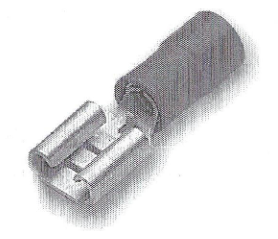
\includegraphics[width=\textwidth]{spade-female} 
        \caption*{Conector tipo "SPADE" hembra}
    \end{minipage}
    \hfill
    \begin{minipage}[b]{0.45\textwidth}
        \centering
        
\includegraphics[width=\textwidth]{torx-symbol} 
        \caption*{Tornillo Torx}
    \end{minipage}
\end{figure}

\vspace{1em}
{\large \textbf{b) Opcionales:}}
\begin{itemize}[label=\CheckmarkBold]
\setlength\itemsep{0em} % Reduce Vspace to make the list fit in the page
\item Una pistola de aire caliente, muy útil para reblandecer pegamentos, detectar fallos que se manifiestan cuando el aparato se sobre calienta, y para aplicar termoretráctil.
\item Una "tercera mano": brazos articulados con npinzas, y a veces una lupa, para soldar cómodamente.
\item Un tester de componentes electrónicos, se encuentran por 15€ en internet.
\item Un magnetizador/desmagnetizador de destornilladores, no son caros y permiten recuperar tornillos difícilmente accesibles...
\item Limas pequeñitas.
\item Pistola de cola caliente.
\item Pelacables.
\item Bomba de aire frío para detectar fallos que aparecen en función de la temperatura.
\item Una regleta con interruptor para apagar rápidamente aparatos "dudosos".
\end{itemize}
\newpage

{\large \textbf{c) Consumibles:}}
\begin{itemize}[label=\CheckmarkBold]
\setlength\itemsep{0em}
\item Varios tipos de pegamento (super glue, epoxy, etc.)
\item Trenza desoldadora.
\item Alambre de estaño de 0,5 y 1mm de diámetro.
\item Grasa.
\item Aceite de vaselina.
\item Alcohol de 90° o isopropílico (para la óptica).
\item Pegamento de "contacto" F2.
\item Lubricante anti-oxidante.
\item Tubo termorretráctil de varios diámetros.
\item Flux de soldadura.
\end{itemize}

\section{El desmontaje: el inicio de la lucha...}
En los electrodomésticos recientes, el desmontaje suele ser una etapa tan difícil como la propia reparación, a veces incluso más. Fabricantes, ingenieros y diseñadores innovan año tras año para asegurarse de que no podamos desmontar sus (¿nuestros?) aparatos.
Utilizar tornillos ocultos bajo las etiquetas, bajo las patas de goma o bajo las piezas de plástico clipadas a veces puede hacernos perder mucho tiempo. También encontrarás tornillos "de seguridad", comprar el destornillador para quitarlos puede valer una fortuna...
A veces, la ausencia de un tornillo significa que tendrás que buscar mucho tiempo para encontrar el lugar adecuado para abrir el aparato sin romperlo.
Y por último, los aparatos moldeados y pegados a veces obligan a utilizar un cúter a lo largo de una ranura para acceder al interior... (batidoras de inmersión Braun y Kenwood, cargadores Apple...) Sólo la perseverancia (y la ayuda de internet) harán que no te rindas antes de empezar...

Tómate tu tiempo para mirar las cosas, para intentar separar cada parte de las demás, para "sentir" cada parte. Intenta "sentir" qué se mueve y qué no se mueve en absoluto, para deducir si hay algún tornillo que no hayas encontrado.

\begin{figure}[h]
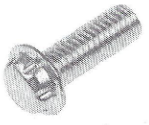
\includegraphics[width=0.2\textwidth]{tornillo-tostadora-phillips} 
\centering
\caption*{\textit{Tornillo extraño encontrado en tostadoras phillips}}
\end{figure}

Cuando se trata de destornilladores de diferentes formas y tamaños, puedes encontrar casi cualquier cosa en ifixit.com, pero una vez más, el precio de la herramienta comparado con el del aparato a reparar detendrá a mucha gente en su camino. Sólo la puesta en común de herramientas puede resolver este problema.\\

{\large \textbf{a) Cómo desatornillar:}}\\

La mayoría de la gente cree saber cómo desenroscar, sin embargo no es raro encontrar casos de gente que lo realizan de mala manera, lo que a veces es destructor para la cabeza del tornillo, y vuelve el desmontaje del aparato imposible sin un taladro de columna para hacer desaparecer la cabeza del tornillo con una broca, cosa que no todo el mundo tiene a su alcance...
Aquí hay un método para evitar esta situación:

\begin{itemize}
\item Elige la herramienta adecuada: fíjate bien en la forma del tornillo
coge un destornillador con la broca que te parezca más adecuada, colócalo en el tornillo y comprueba que no hay holgura entre la punta y el tornillo.
La punta debe acoplarse perfectamente al tornillo, casi no se debe ver holgura.
\item A continuación, aconsejo mantener un buen apoyo vertical sobre el tornillo y dar un pequeño golpe seco de rotación, en el sentido inverso de las agujas del reloj (excepto en casos raros: rotnillo sobre el eje de un motor, en algunas piezas de bici, máquinas de coser...)
De esta manera evitaremos al máximo que el destornillador "salte" sobre el tornillo y deteriore la cabeza, haciendo su extracción cada vez más difícil.
\end{itemize}
\begin{figure}[h]
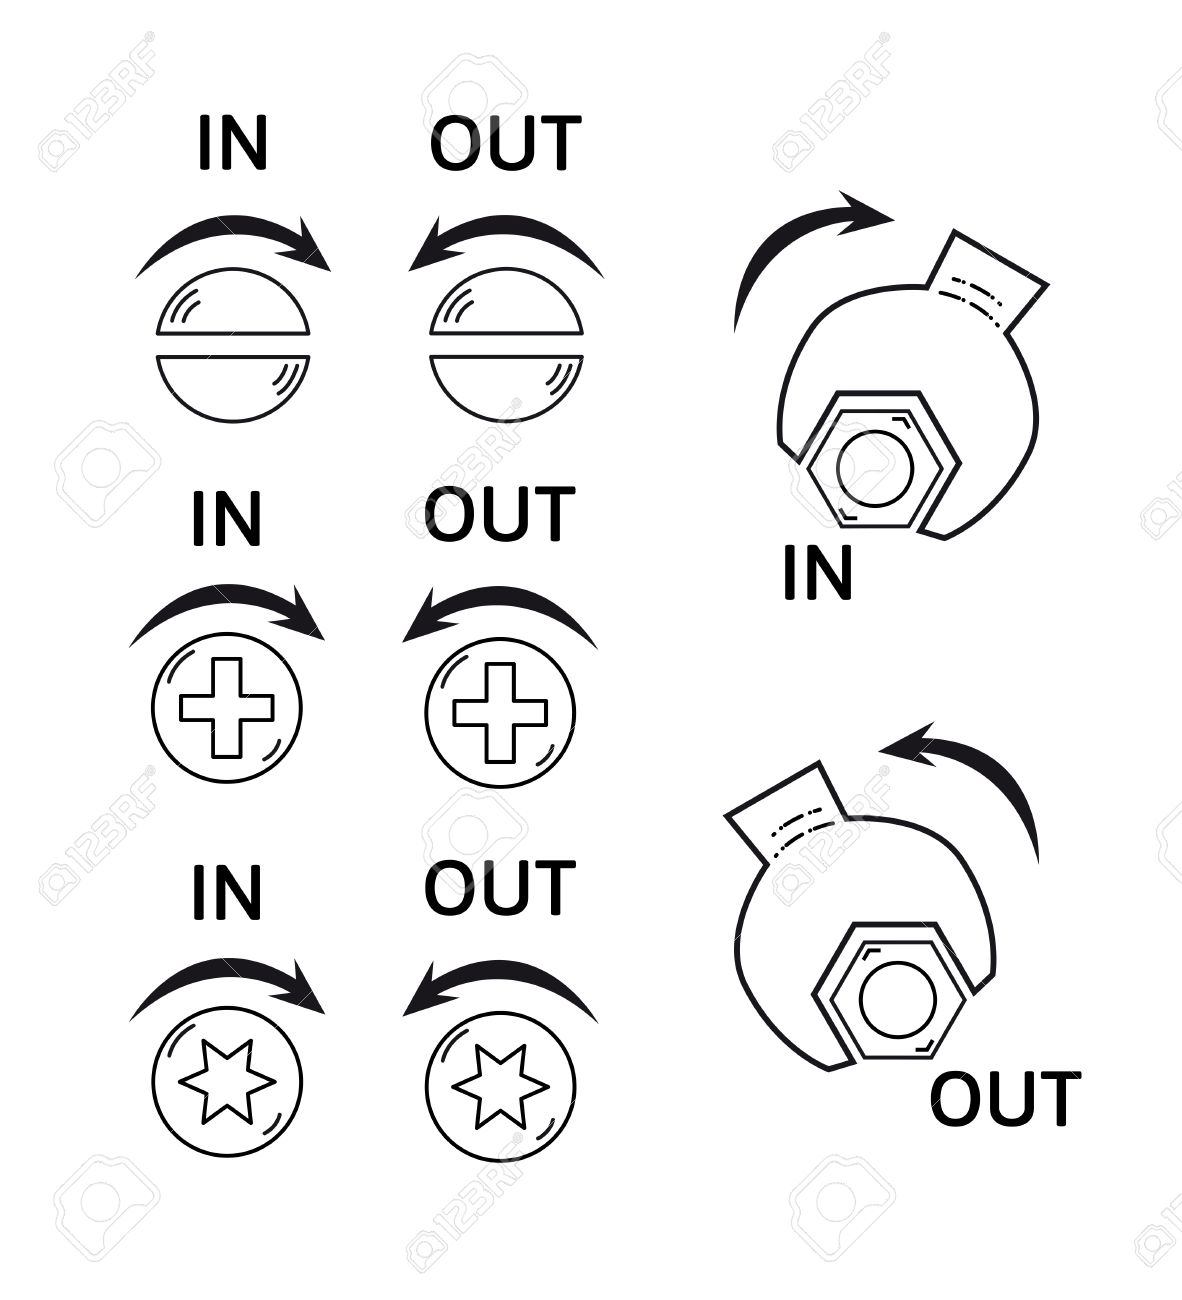
\includegraphics[width=0.4\textwidth]{diagrama-righty-tighty} 
\centering
\caption*{\textit{Righty tighty, lefty loosey ;)}}
\end{figure}

{\large \textbf{b) Los conectores:}}\\
Cuando desmontes u aparato, a menudo deberás desconectar placas electrónicas conectadas entre ellas, o conectadas por algún tipo de cable con conectores. A veces es suficiente estirar (a veces incluso con bastante fuerza), pero debes tener cuidado con ciertos conectores. Mira bien si no hay algún mecanismo de cerrojo como para los modelos encontrados abajo. A menudo, el clip de desconexión es de un color distinto al resto del conector.

\begin{itemize}


\begin{figure}[h]
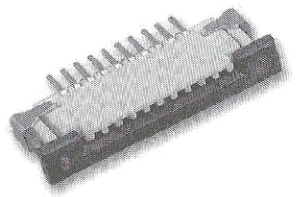
\includegraphics[width=0.4\textwidth]{conector-deslizante} 
\centering
\caption*{\textit{Modelo de conector deslizante}}
\end{figure}
\item Modelo deslizante: hay que tirar ligeramente hacia el exterior del mecanismo para desconectar el cable.
\begin{figure}[h]
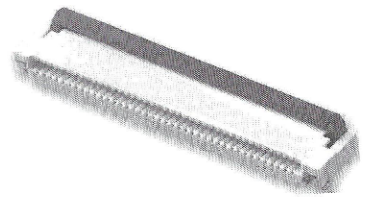
\includegraphics[width=0.4\textwidth]{conector-basculante} 
\centering
\caption*{\textit{Modelo de conector basculante}}
\end{figure}
\item Modelo basculante: hay que levantar delicadamente la parte superior del mecanismo, a veces del lado del cable, menos frecuentemente, como en la foto, del lado opuesto.
\end{itemize}

En ambos casos, usa las uñas o un destornillador plano muy fino y tira con cuidado, cuando se rompe un conector de este tipo suele ser bastante difícil de remplazar.
\newpage

\section{Historial y origen del problema}

Es muy importante enterarse del historial de un fallo para deducir de donde puede (o no) venir.\\

{\large \textbf{a) El aparato se ha caído o ha recibido un golpe}}\\

Si es así, es muy probable que algo se haya roto en el interior y esté causando una avería,
causando un mal funcionamiento: una placa de circuito rota o agrietada, un conector, un cable o una soldadura arrancados, un trozo de plástico roto...
El problema suele ser visible, sólo tienes que mirar con atención.
Con la práctica, serás capaz de ver enseguida qué falla.\\

{\large \textbf{b) El problema empeora cada día}}\\

Si la avería se ha producido gradualmente, hay que pensar en algo que evoluciona con el tiempo, acumulación de polvo, componentes al final de su vida útil, etc.
Según el tipo de electrodoméstico y avería, debe dar prioridad a la revisión de las partes que necesitan una limpieza regular:

\begin{itemize}

\item Los elementos ópticos: bloque lector de un CD/DVD
\item Los elementos y componentes que se calientan, y aquellos que los enfrían: disipadores y ventiladores de un ordenador portátil
\item Las partes mecánicas: barqueta de un lector CD/DVD, correas, engranajes...
\item Los contacos eléctricos: muelles de contacto de las pilas, interruptores, escobillas del motor...
\end{itemize}

{\large \textbf{c) El fallo aparece después de la puesta en marcha}}\\

En este caso, se trata probablemente de un elemento o componente electrónico cuyo estado cambia en función de su temperatura, por ejemplo
una unión soldada (porque el metal se dilata con la temperatura).

Puede tratarse de un componente mecánico cuya lubricación (demasiado antigua) mejora volviéndose más fina al aumentar la temperatura.

O al contrario, un componente eléctrico que funciona mal en cuanto sube la
temperatura.\\
\newpage
{\large \textbf{d) Problema intermitente}}\\

Si el problema aparece y desaparece sin ninguna razón en particular, o aparece cuando mueves el aparato, probablemente se trate de un mal contacto de una unión soldada o un conector.\\

{\large \textbf{e) El problema aparece en funciones específicas}}\\

Si el aparato se enciende, entiende comprender qué es lo que funciona y lo que no, ayudará mucho al diagnóstico que sigue.
Por ejemplo, prueba varios programas de la lavadora, si no deja elegir la función de centrifugado o vaciado de forma independiente a un programa, intenta ver si estas funciones pueden ser parte del problema (fallo de la bomba, fallo del elemento calentador ...)
A veces existen programas de diagnóstico, sobre todo en lavadoras y lavavajillas.
\newpage
